\begin{figure*}[t]
  \centering
  \resizebox{0.94\textwidth}{!}{% Method overview. First draft generated with the local Codex CLI (paper/codex/pipeline), then
% revised by hand: layout grid, overlaps, labels. Thumbnails are real buffers of the final Hotdog model.
\begin{tikzpicture}[
  x=1cm,y=1cm,
  font=\sffamily\fontsize{7.4}{8.6}\selectfont,
  line width=0.65pt,
  >={Stealth[length=4pt]},
  light/.style={draw=orange!70!black,fill=orange!8,rounded corners=2pt},
  camera/.style={draw=blue!60!black,fill=blue!6,rounded corners=2pt},
  learned/.style={draw=green!45!black,fill=green!8,rounded corners=2pt},
  lightflow/.style={->,draw=orange!70!black},
  cameraflow/.style={->,draw=blue!60!black},
  mergeflow/.style={->,draw=black!75},
  label/.style={fill=white,inner sep=1.2pt,align=center},
  thumb/.style={draw=gray!65,inner sep=0pt,outer sep=0pt},
  title/.style={font=\sffamily\bfseries\fontsize{7.8}{9}\selectfont},
  stage/.style={align=left,anchor=north west,inner sep=0pt,font=\sffamily\fontsize{7}{8}\selectfont}
]
\path[use as bounding box] (0,0) rectangle (17.4625,6.35);

% ---------------------------------------------------------------- light pass
\node[title,anchor=west,text=orange!70!black] at (0.05,6.18) {Light pass};
\node[light,minimum width=2.40cm,minimum height=1.06cm,align=center] (gaussians) at (1.30,4.62)
  {\textbf{3D Gaussians}\\[3pt]$\{\mu_i,\Sigma_i,o_i,\mathbf b_i,\mathbf f_i\}$};
\node[learned,minimum width=1.55cm,minimum height=0.43cm] (phi) at (1.30,5.62) {$\boldsymbol\phi$-MLP};
\draw[lightflow] (gaussians.north) -- (phi.south);
\draw[lightflow] (phi.east) -- (2.55,5.62) -- (2.55,6.02) -- (4.90,6.02) -- (4.90,5.88);
\node[label] at (3.72,6.20) {rasterize from the light $\mathbf p$};

\draw[light] (2.94,3.52) rectangle (6.88,5.88);
\node[title] at (4.91,5.70) {Light-space atlas};
\node[thumb] at (3.93,4.92) {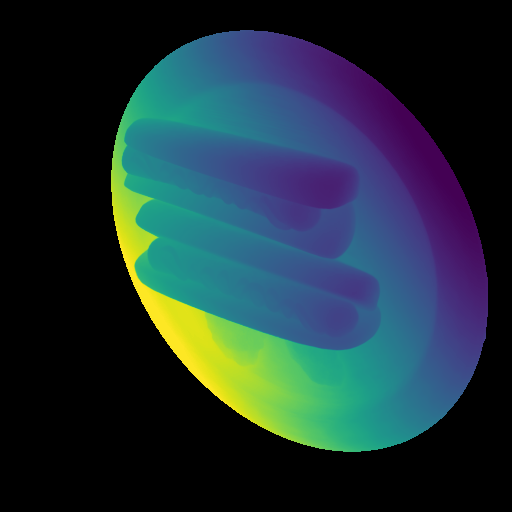
\includegraphics[width=1.22cm,height=1.22cm]{figures/decomp_hotdog/atlas_depth.png}};
\node[thumb] at (5.86,4.92) {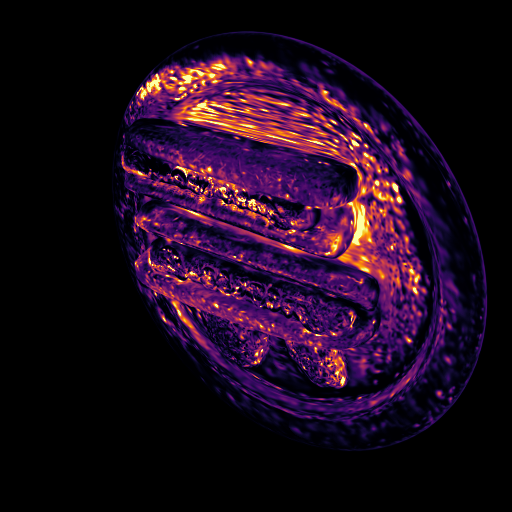
\includegraphics[width=1.22cm,height=1.22cm]{figures/decomp_hotdog/atlas_flux.png}};
\node[align=center] at (3.93,4.08) {depth $M_1,M_2$};
\node[align=center] at (5.86,4.08) {flux $\boldsymbol\Phi$};
\node at (4.91,3.72) {$\mathbf A(u)=\sum_i w_i(u)\,[\boldsymbol\phi_i,\,z_i,\,z_i^2,\,1]$};

\draw[lightflow] (6.88,4.92) -- (7.55,4.92);
\node[align=center] at (7.21,4.52) {blur\\$\downarrow 2$};
\node[title,anchor=south] at (8.50,5.62) {Pyramid $\{\mathbf A_k\}_{k<K}$};
\node[thumb] at (8.25,4.95) {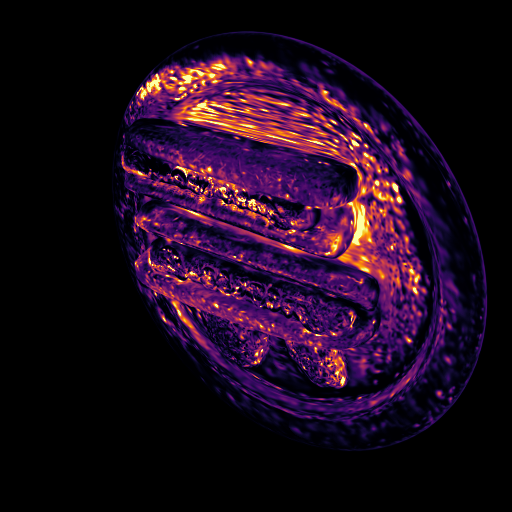
\includegraphics[width=1.22cm,height=1.22cm]{figures/decomp_hotdog/atlas_flux.png}};
\node[thumb] at (8.70,4.66) {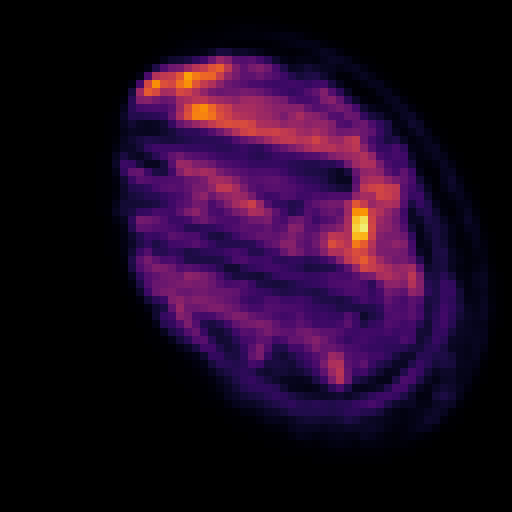
\includegraphics[width=0.90cm,height=0.90cm]{figures/decomp_hotdog/atlas_flux_level3.png}};
\node[thumb] at (9.06,4.42) {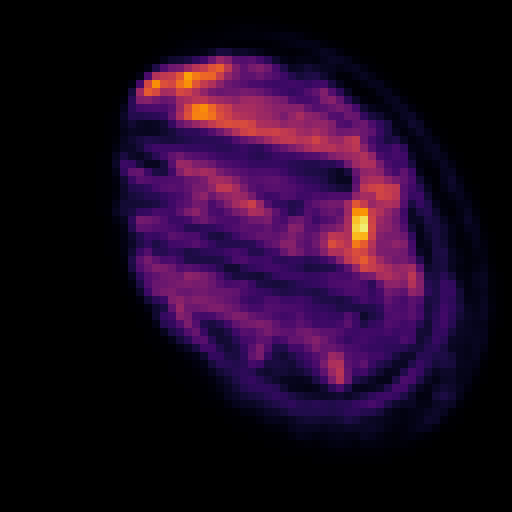
\includegraphics[width=0.62cm,height=0.62cm]{figures/decomp_hotdog/atlas_flux_level3.png}};

% ---------------------------------------------------------------- camera pass
\node[title,anchor=west,text=blue!60!black] at (0.05,3.38) {Camera pass};
\node[camera,minimum width=2.40cm,minimum height=1.20cm,align=center] (receivers) at (1.30,2.42)
  {\textbf{Receivers $\mathbf x$}\\[2pt]Gaussian centers (II)\\or pixels (III)};
\node[camera,minimum width=5.90cm,minimum height=1.20cm,inner sep=2pt,align=center] (gather) at (6.02,2.42)
  {\textbf{Gather at $u(\mathbf x)$, every level $k$}\\[2pt]
   $\mathbf q_k=[M_{0,k},\,t_k,\,\delta_k,\,\log\eta_k,\,V_k],\ \ \boldsymbol\Phi_k$\\[2pt]
   $V_k=1-M_{0,k}\,G(t_k-\beta)$};
\draw[cameraflow] (receivers.north) -- (1.30,3.24) -- (7.90,3.24) -- (7.90,4.32);
\node[label] at (4.85,3.24) {project into the light: $(u(\mathbf x),z(\mathbf x))$};
\draw[cameraflow] (8.70,4.20) -- (8.70,3.03);
\node[label,anchor=west] at (8.78,3.62) {sample};

% ---------------------------------------------------------------- learned heads
\node[title,anchor=west,text=green!45!black] at (10.05,6.18) {Shading};
\node[learned,minimum width=4.85cm,minimum height=1.05cm,align=center] (visibility) at (12.50,5.42)
  {\textbf{visibility $\mathcal G$}\\[2pt]$V=\sigma\big(\mathrm{logit}\,V_0+\mathcal G(\mathbf Q,\mathbf f,\mathbf n\!\cdot\!\mathbf l)\big)$};
\node[learned,minimum width=4.85cm,minimum height=1.05cm,align=center] (transfer) at (12.50,4.14)
  {\textbf{transfer $\mathcal K$}\\[2pt]$L_{\mathrm{tr}}=\sum_k\mathbf W_k\,\boldsymbol\Phi_k$, \ $\mathbf W_k$ from $\mathbf Q$};
\node[learned,minimum width=4.85cm,minimum height=1.05cm,align=center] (material) at (12.50,2.86)
  {\textbf{local material}\\[2pt]$\rho=\mathrm{MLP}(\mathbf f,\mathbf n,\mathbf l,\mathbf v,\mathbf h,\mathbf r)$, lobes $s$};
\draw[draw=blue!60!black] (gather.east) -- (9.70,2.42) -- (9.70,5.42);
\draw[cameraflow] (9.70,5.42) -- (visibility.west);
\draw[cameraflow] (9.70,4.14) -- (transfer.west);
\draw[cameraflow] (9.70,2.86) -- (material.west);
\fill[blue!60!black] (9.70,4.14) circle (0.65pt);
\fill[blue!60!black] (9.70,2.86) circle (0.65pt);

\node[thumb] (visimage) at (16.20,5.42) {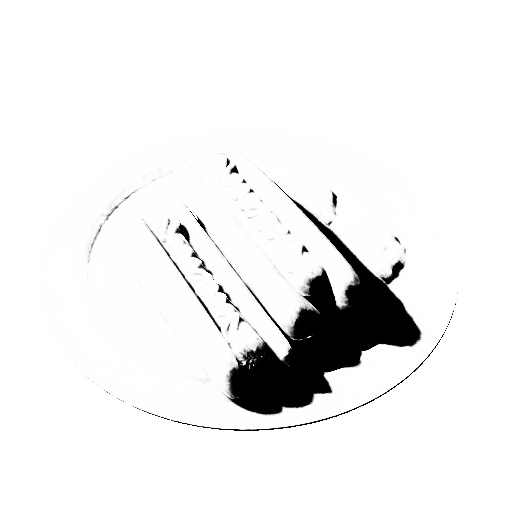
\includegraphics[width=1.12cm,height=1.12cm]{figures/decomp_hotdog/visibility.png}};
\node[thumb] (trimage) at (16.20,4.14) {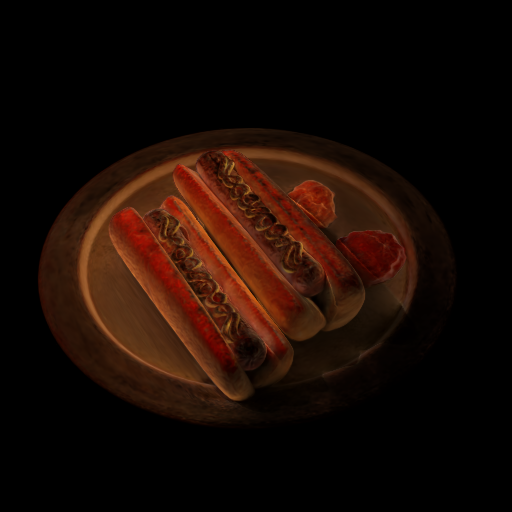
\includegraphics[width=1.12cm,height=1.12cm]{figures/decomp_hotdog/transfer.png}};
\node[thumb] (matimage) at (16.20,2.86) {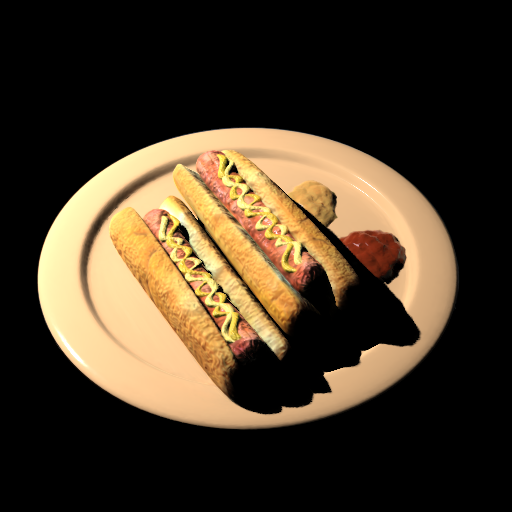
\includegraphics[width=1.12cm,height=1.12cm]{figures/decomp_hotdog/local.png}};
\draw[draw=green!45!black] (visibility.east) -- (visimage.west);
\draw[draw=green!45!black] (transfer.east) -- (trimage.west);
\draw[draw=green!45!black] (material.east) -- (matimage.west);

% ---------------------------------------------------------------- radiance
\draw[draw=black!75] (15.25,5.42) -- (15.25,2.03);
\fill[black!75] (15.25,5.42) circle (0.65pt);
\fill[black!75] (15.25,4.14) circle (0.65pt);
\fill[black!75] (15.25,2.86) circle (0.65pt);
\node[draw=black,fill=white,rounded corners=2pt,minimum width=15.0cm,minimum height=0.58cm,align=center] (shading) at (7.62,1.45)
  {$L(\mathbf x)=\bar E(\mathbf x)\big[\,V\rho+V_0\,s+\textstyle\sum_k\mathbf W_k\boldsymbol\Phi_k\big],\qquad \bar E(\mathbf x)=\mathbf I/\|\mathbf p-\mathbf x\|^2$};
\draw[mergeflow] (15.25,2.03) -- (15.25,1.74);
\node[thumb] (output) at (16.55,1.45) {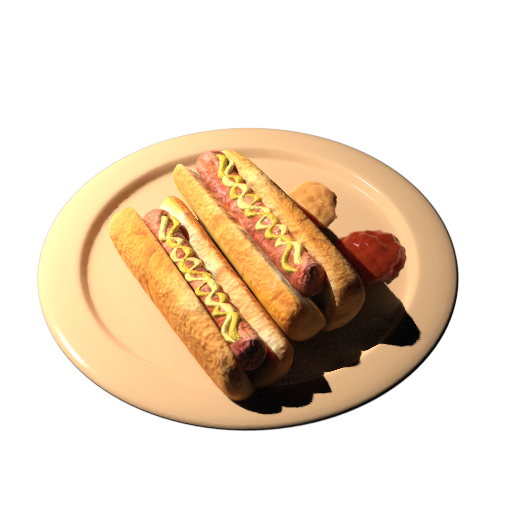
\includegraphics[width=1.05cm,height=1.05cm]{figures/decomp_hotdog/ours.png}};
\draw[mergeflow] (shading.east) -- (output.west);

% ---------------------------------------------------------------- schedule (8k : 22k : 8k)
\fill[gray!10] (0.06,0.02) rectangle (3.7116,0.98);
\fill[blue!8] (3.7116,0.02) rectangle (13.7534,0.98);
\fill[green!8] (13.7534,0.02) rectangle (17.405,0.98);
\draw[draw=gray!60,rounded corners=2pt] (0.06,0.02) rectangle (17.405,0.98);
\draw[draw=gray!60] (3.7116,0.02) -- (3.7116,0.98);
\draw[draw=gray!60] (13.7534,0.02) -- (13.7534,0.98);
\node[stage,text width=3.50cm] at (0.16,0.90)
  {\textbf{I. Geometry warm-up} (8k)\\no networks; target $Y^{1/\gamma}\!\to\!Y$};
\node[stage,text width=9.80cm] at (3.84,0.90)
  {\textbf{II. Joint training} (22k)\\linear-radiance loss; Gaussian receivers; densification};
\node[stage,text width=3.55cm] at (13.86,0.90)
  {\textbf{III. Refinement} (8k)\\frozen geometry; pixel receivers; display-domain loss};
\end{tikzpicture}
}
  \caption{\textbf{Overview.}
For every light, the Gaussians are rasterized once from the light; each deposits learned flux features $\boldsymbol\phi_i$ and its depth moments with the compositing weight that equals the fraction of light it intercepts (\cref{eq:atlas}).
A receiver projects into the light, gathers multi-scale statistics and flux from the pyramid, and is shaded by a residual on the moment shadow test, transfer kernels applied linearly to the gathered flux features, and a local material.
Thumbnails: actual buffers of our Hotdog model on a test view. Bottom: the schedule of \cref{sec:optimization}.}
  \label{fig:pipeline}
\end{figure*}
